\section{Оптимизация направленности ФАР: основные понятия, постановка задач, проблемы и методы решения}
\subsection{Основные понятия}
\begin{frame}[plain, noframenumbering]
    \begin{center}
        \Huge
        Оптимизация направленности ФАР: основные понятия, постановка задач, проблемы и методы решения
    \end{center}
\end{frame}

\begin{frame}[plain, noframenumbering]
    \frametitle{Основные понятия}
    \begin{center}
        \begin{figure}
            \begin{minipage}[h]{0.42\linewidth}
                \center{\includegraphics[width=1\linewidth]{2x2bve.eps} \\ а)}
            \end{minipage}
            \hfill
            \begin{minipage}[h]{0.42\linewidth}
                \center{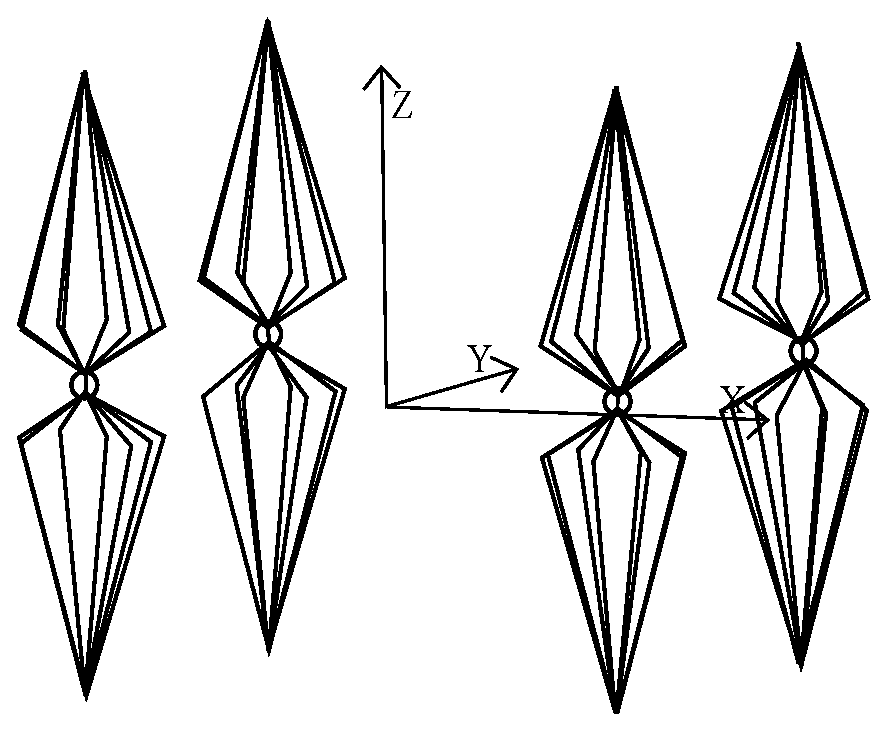
\includegraphics[width=0.6\linewidth]{2x2bvd.eps} \\ б)}
            \end{minipage}
            \begin{minipage}[h]{0.42\linewidth}
                \center{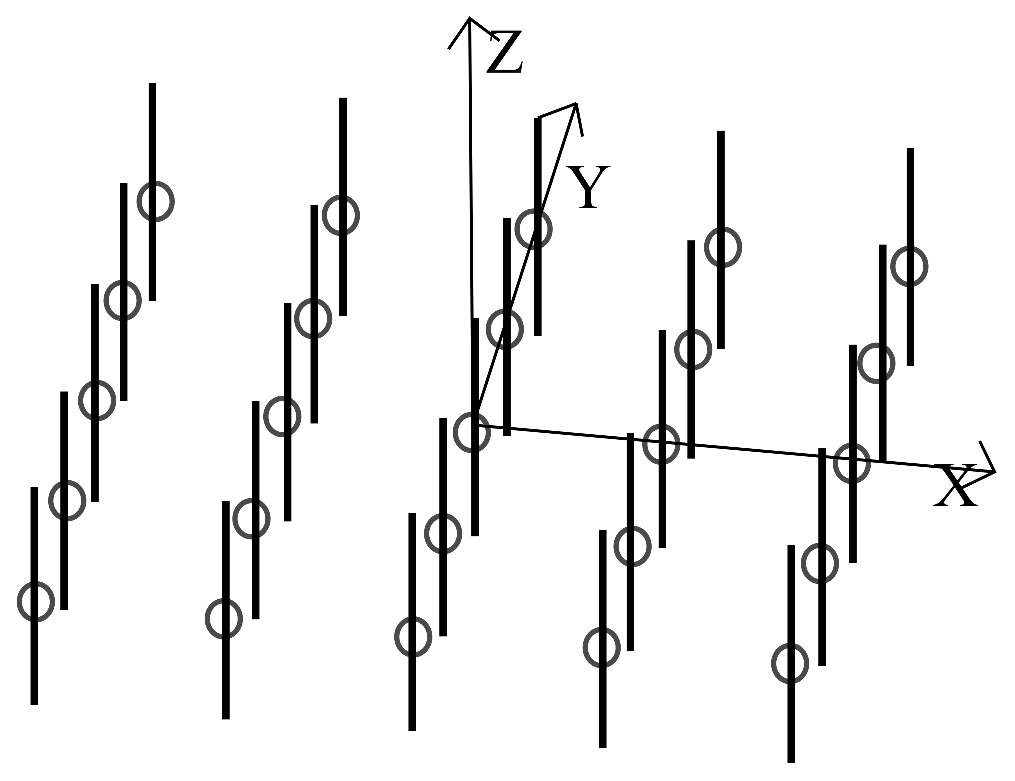
\includegraphics[width=0.6\linewidth]{5x5VWD.eps} \\ в)}
            \end{minipage}
            \hfill
            \begin{minipage}[h]{0.42\linewidth}
                \center{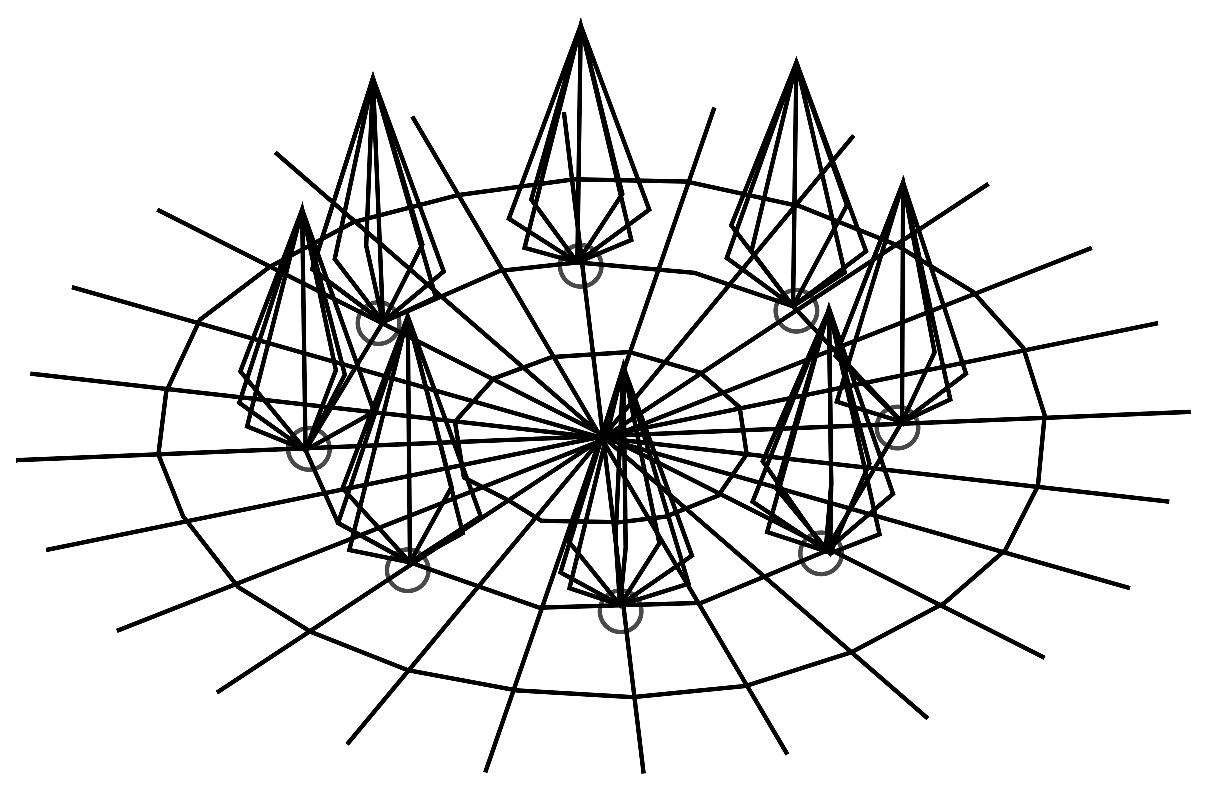
\includegraphics[width=0.9\linewidth]{r8.eps} \\ г)}
            \end{minipage}
            \label{ris:bve_bvd}
            \caption{ФАР различных конфигураций}
        \end{figure}

    \end{center}
    \footnotesize { \textbf{Юрков А.С.:} Оптимизация возбуждения передающих фазированных антенных решеток декаметрового диапазона длин волн. ОНИИП, Омск (2014)\\
    \textbf{Fuchs B.:} Application of convex relaxation to array synthesis problems. IEEE, P.~634-640, 2014.
    }
\end{frame}

\subsection{Постановка в вещественных числах}
\begin{frame}
    \frametitle{Постановка в вещественных числах}

    \begin{equation}
        \begin{cases}
           \textbf{x}^{T}\textbf{Gx} \rightarrow \max,\\
           0 \leq \textbf{x}^{T}\textbf{H}^{(1)}\textbf{x} \leq 1,\\
           ...\\
           0 \leq \textbf{x}^{T}\textbf{H}^{(n)}\textbf{x} \leq 1,\\
          \textbf{x} \in \mathbb{R}^{2n}.\\
         \end{cases}
         \label{eq:task3}
    \end{equation}
    
    
\vspace{8em}


\footnotesize { \textbf{Еремеев А.В., Тюнин Н.Н., Юрков А.С.:} Non-Convex Quadratic Programming Problems in Short Wave Antenna Array Optimization. MOTOR 2019 (11584) }
\end{frame}

\section{Анализ структуры локальных оптимумов}
\subsection{Постановка задачи}
\begin{frame}
    \frametitle{Постановка задачи}
    \begin{block}{Метод штрафных функций}
        \begin{equation}
               \textbf{x}^{T}\textbf{Gx} - r\cdot \sum_{k=1}^n
               \left( \min\left(0,\textbf{x}^{T}\textbf{H}^{(k)}\textbf{x}\right) +
               \min\left(0,1-\textbf{x}^{T}\textbf{H}^{(k)}\textbf{x}\right)\right)^4 \rightarrow
               \max
             \label{eq:task4}
        \end{equation}
    \end{block}

    \begin{block}{Необходимые условия локальной оптимальности}
        \begin{equation}
            \begin{cases}
               \textbf{x}_0^T\textbf{G}\textbf{x}_0 + 2\textbf{x}_0^T\textbf{G}\textbf{y} \rightarrow \max,\\
               0 \leq \textbf{x}_0^T\textbf{H}^{(1)}\textbf{x}_0 + 2\textbf{x}_0^T\textbf{H}^{(1)}\textbf{y} \leq 1,\\
               ...\\
               0 \leq \textbf{x}_0^T\textbf{H}^{(n)}\textbf{x}_0 + 2\textbf{x}_0^T\textbf{H}^{(n)}\textbf{y} \leq 1,\\
              \textbf{y} \in \mathbb{R}^{2N}.\\
             \end{cases}
             \label{eq:task5}
        \end{equation}
    \end{block}
\end{frame}

%------------------------------------------------
\subsection{Вычислительный эксперимент}
\begin{frame}
    \frametitle{ Вычислительный эксперимент }
    Цели эксперимента
    \begin{itemize}
      \item Исследование структуры локальных оптимумов
      \item Сравнение эффективности работы различных алгоритмов
      \item Исследование возможностей ФАР в разных условиях
    \end{itemize}
    Исследуемые алгоритмы
    \begin{itemize}
      \item Градиентный подъем
      \item BARON
      \item Дифференциальная эволюция
    \end{itemize}
    Детали эксперимента
    \begin{itemize}
      \item Антенный моделировщик NEC2
      \item Направление оптимизации $70^{\circ}:45^{\circ}$
    \end{itemize}
\end{frame}

%------------------------------------------------
\subsection{Структура локальных оптимумов}
\begin{frame}
    \frametitle{Структура локальных оптимумов}
    \begin{table}[!h]
    \centering
    \begin{tabular}{|l | c | c | c | c |}
        \hline
        \textbf{ФАР} & \textbf{$M$} & \textbf{$M_{ne}$} & \textbf{$M_{f}$} & \textbf{$M_{y\approx0}$}\\
        \hline
        ШВИ 2x2 & 18368 & 4 & 1 & 4\\
        ШВД 2x2 & 7678  & 4 & 1 & 4\\
        СВД 2x2  & 523  & 1 & 1 & 1\\
        СВД' 3x3  & 14  & 14 & 3 & 1\\
        ШВИ 3x3 & 1070  & 3 & 1 & 3\\
        ШВД 3x3 & 41  & 4 & 4 & 1\\
        Кольц. 8 & 124  & 9 & 2 & 9\\
        Кольц. 16 & 11  & 6 & 1 & 6\\
        \hline
    \end{tabular}
    \label{tab:structure}
\end{table}

\begin{block}{Фазовая симметрия}
    \begin{equation}
         \textbf{i} \to e^{\textit{\textbf{j}}\phi}\textbf{i}
    \end{equation}
\textbf{Еремеев А.В., Юрков А.С.:} On Symmetry Groups of Some Quadratic Programming Problems~// MOTOR 2020. Shpringer, 2020. Vol.~12095.
\end{block}
\end{frame}

%------------------------------------------------

\begin{frame}
    \frametitle{Сравнение результатов оптимизации градиентного подъема и решателя BARON}
    \begin{table}
\centering
\begin{tabular}{|c|c|c|c c|c c|}
    \hline
    \multirow{2}{*}{\textbf{ФАР}} & \multirow{2}{*}{$\lambda_{min}$} & \multirow{2}{*}{$\sqrt{\frac{N}{\lambda_{\min}}}$} & \multicolumn{2}{c}{\textbf{Град.}} & \multicolumn{2}{|c|}{\textbf{BARON}}\\
    & & & \textbf{$\textbf{F}$} & \textbf{t, c} & \textbf{$\textbf{F}$} & \textbf{t, c} \\
    \hline
    ШВИ 2х2 & 0.0215 & 13.6 & 138.2 & \textbf{0.054} & \textbf{139.2} & 0.12 \\
    ШВИ 3х3 & 0.0177 & 70 & 575.7 & 0.93 & \textbf{580.6} & \textbf{0.34} \\
    ШВД 2х2 & 0.009 & 21 & 459.7 & \textbf{0.13} & \textbf{463.6} & 0.27 \\
    ШВД 3х3 & 0.0013 & 6767 & 915 & 24.4 & \textbf{925} & \textbf{0.34}  \\
    СВД 2х2 & $2\cdot10^{-3}$ & 44& 357 & 1.9 & \textbf{361} & \textbf{0.16} \\
    СВД' 3х3 & 0.0008 & $1\cdot10^4$& 664 & 71 & \textbf{1153} & \textbf{1.48} \\
    Кольц. 8 & $3\cdot10^{-3}$ & 154 & 217 & 8.06 & \textbf{218} & \textbf{0.23} \\
    Кольц. 16 & $6.7\cdot10^{-4}$ & $1.2\cdot10^{6}$& 727 & 90.9 & \textbf{734} & \textbf{1.37} \\
    \hline
\end{tabular}
\label{tab:results}
\end{table}

$\sqrt{\frac{N}{\lambda_{\min}}}$ - оценка сверху евклидовой нормы.
\end{frame}

\begin{frame}
    \frametitle{Кластеры решений}

    \begin{figure}
    \centering
        \begin{minipage}[h]{0.6\linewidth}
                \center{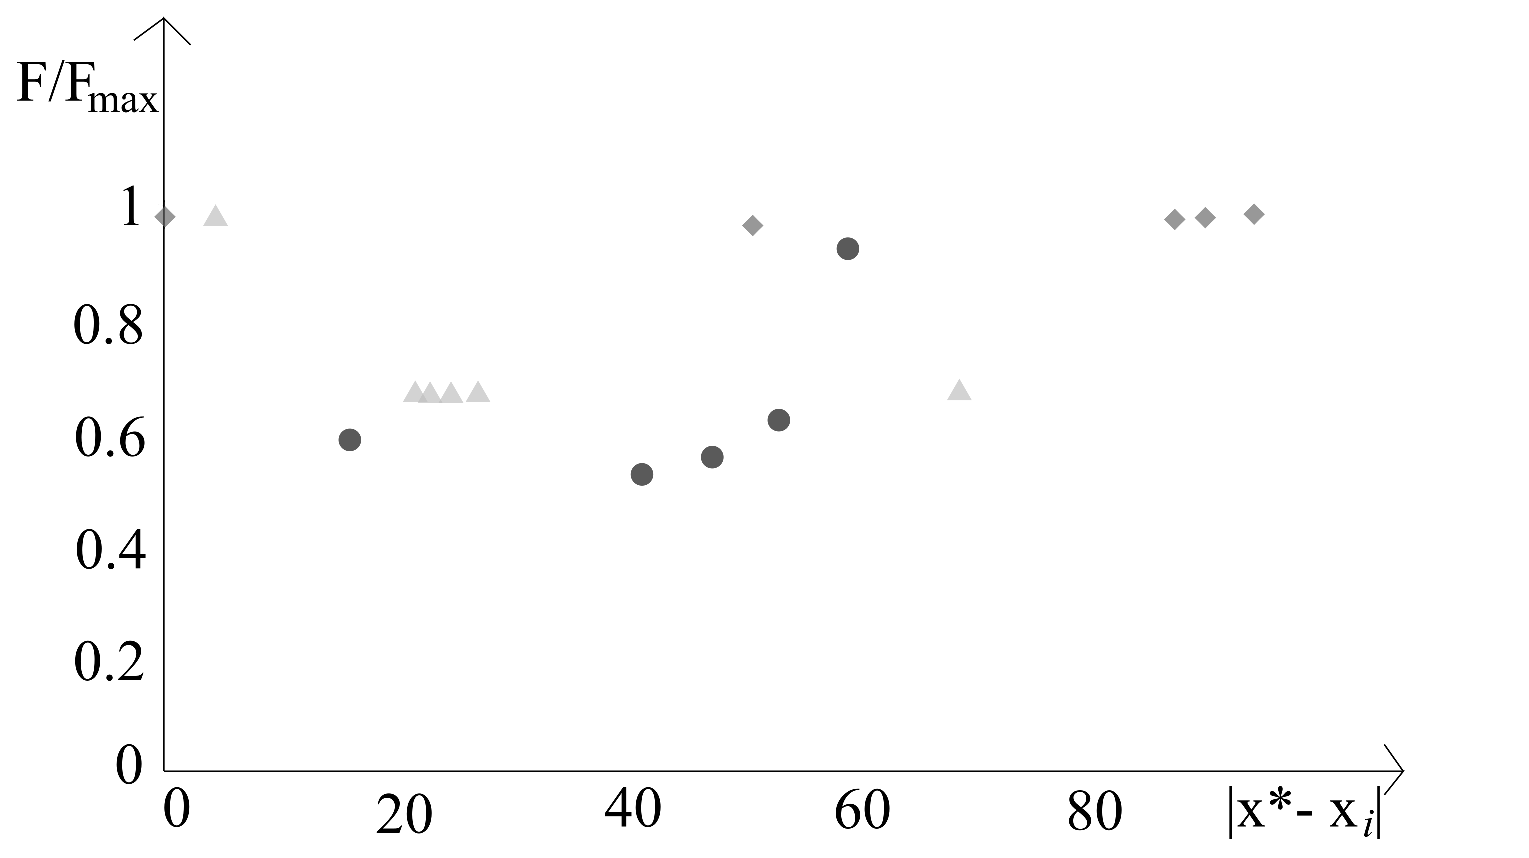
\includegraphics[width=0.9\linewidth]{fit_dist.eps}  \\ а) }
        \end{minipage}
        \begin{minipage}[h]{0.6\linewidth}
                \center{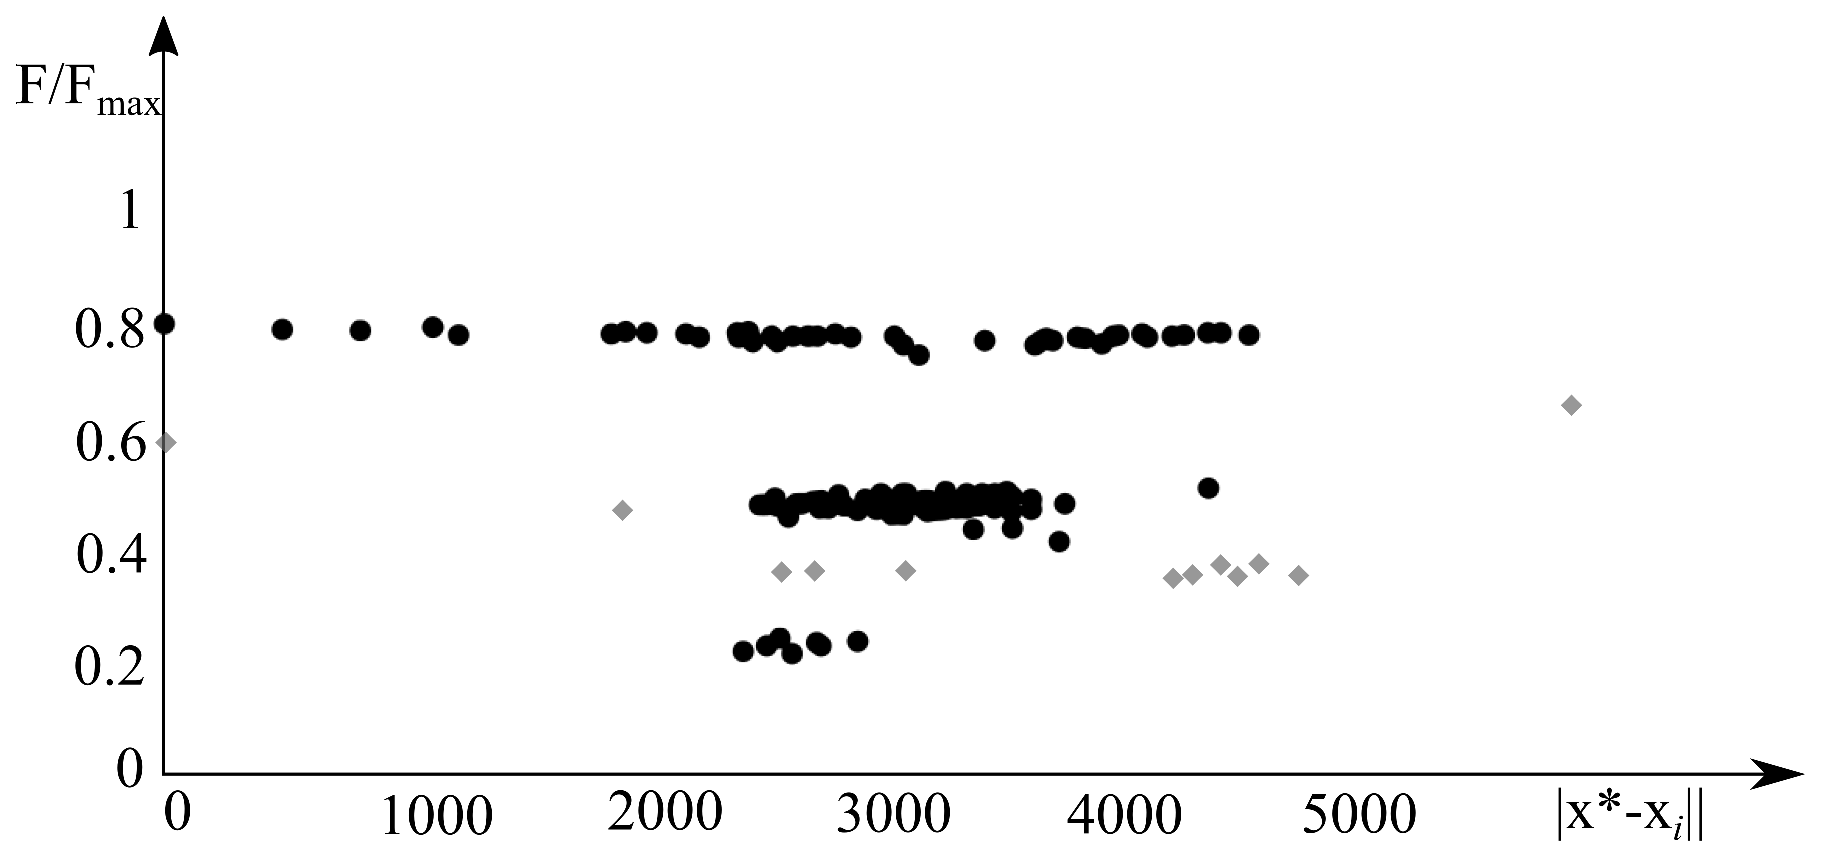
\includegraphics[width=0.9\linewidth]{fit_dist_2x2.eps}  \\ б) }
        \end{minipage}
        \vspace{0.7em}
        \caption{Структура множества найденных решений для задач ШВИ, ШВД, СВД (а) и СВД' (б)}
        \label{ris:fit_dist}
    \end{figure}

\end{frame}

%------------------------------------------------
\subsection{Экспериментальная проверка устойчивости решений}
\begin{frame}
    \frametitle{Экспериментальная проверка устойчивости решений}
    \begin{figure}[h]
    \centering
    \center{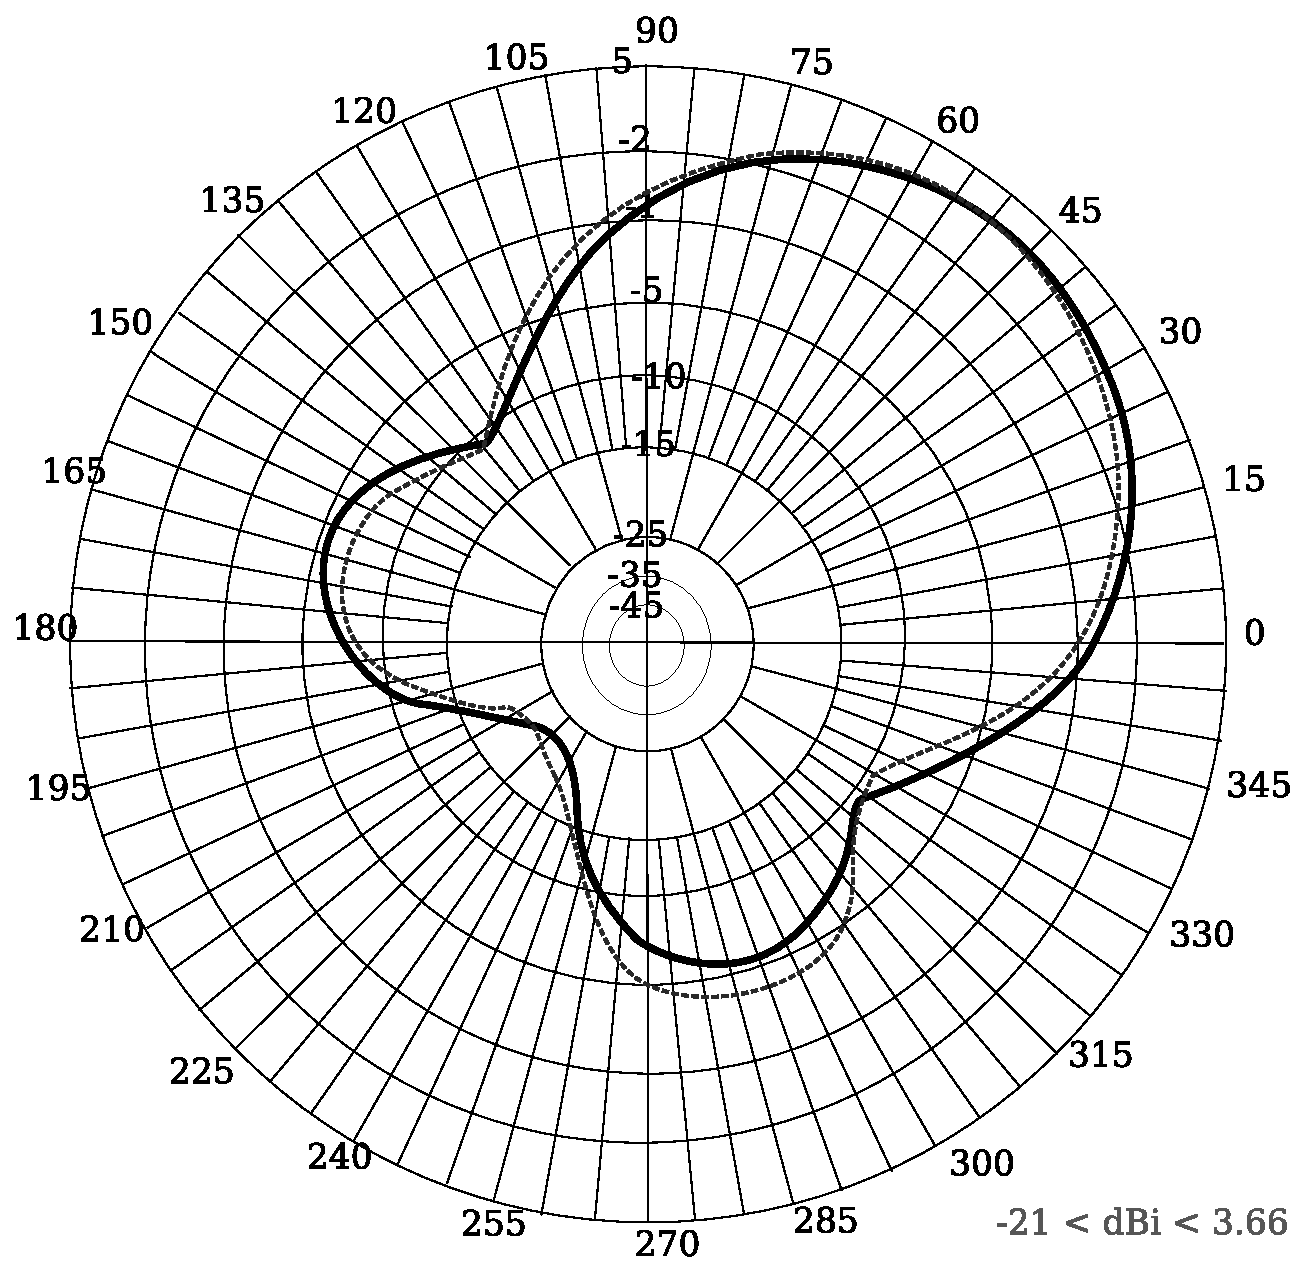
\includegraphics[width=0.5\linewidth]{stability.eps} }
    \vspace{0.7em}
    \caption{Диаграммы направленности для ШВИ~2x2 при оптимизации в направлении 70:45 (сплошная линия) и 70:50 (пунктир)}
    \label{ris:bve_comp}
    \end{figure}
\end{frame}

%------------------------------------------------

\subsection{Дифференциальная эволюция}
\begin{frame}
    \frametitle{Дифференциальная эволюция}
    \begin{figure}
    \center{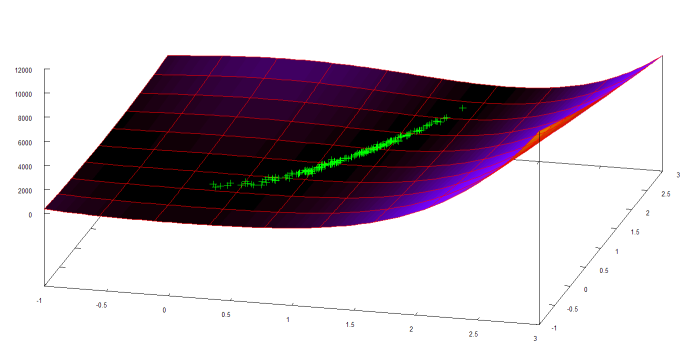
\includegraphics[width=0.7\linewidth]{de.png}}
    \caption{Поиск минимума функции Розенброка методом ДЭ}
    \label{ris:rosenbroke}
    \end{figure}
    \begin{itemize}
      \item $v=v_{1}+f\cdot (v_{2}-v_{3}),$
            где $v_1, v_2, v_3$ - случайные особи из текущей популяции, не равные друг другу.
      \item Гибридный алгоритм с градиентным методом.
      \item Адаптация алгоритма для запуска на GPU.
    \end{itemize}
\end{frame}

%------------------------------------------------

\section{Исследование возможностей ФАР в разных условиях}
\subsection{Исследование радиочастотных зависимостей}
%------------------------------------------------

\begin{frame}
    \frametitle{Исследование радиочастотных зависимостей}
\begin{figure}
\center{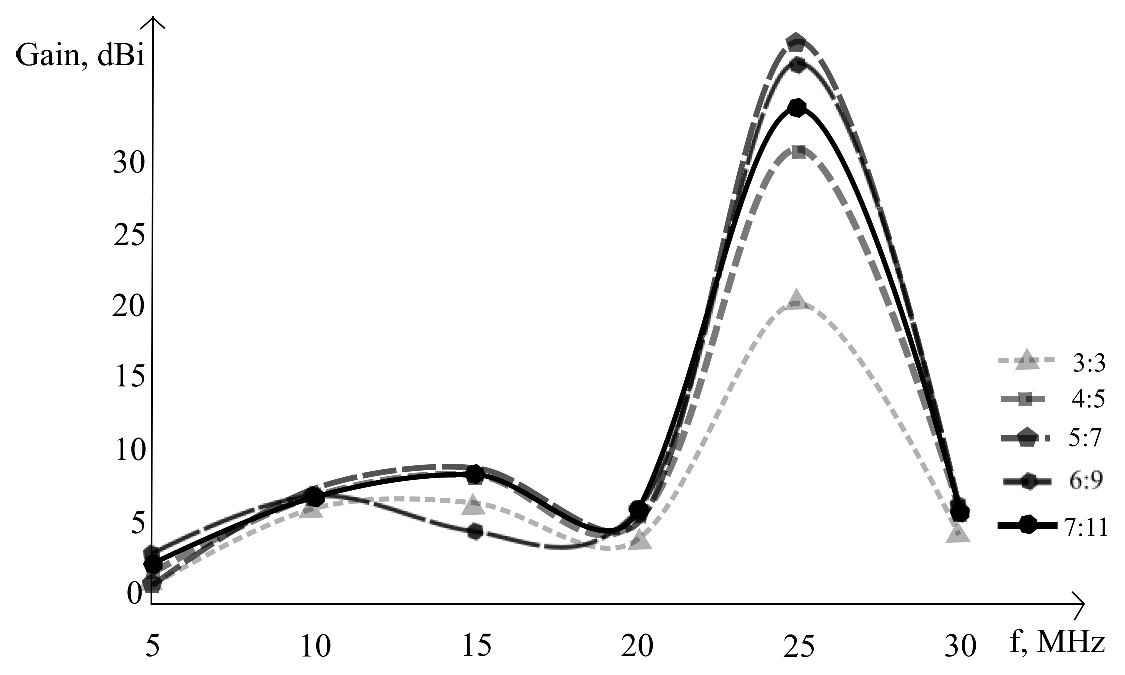
\includegraphics[width=0.5\linewidth]{ring_f_gains.eps}}
\label{ris:paa_gains}
\caption{Сравнение усиления ФАР и одиночного излучателя на различных частотах.}
\end{figure}

\begin{figure}
\begin{minipage}[h]{0.4\linewidth}
\center{
\includegraphics[width=1\linewidth]{r8_1_25_5x7.png}} a)
\end{minipage}
\hfill
\begin{minipage}[h]{0.4\linewidth}
\center{
\includegraphics[width=1\linewidth]{r8_25_5x7.png}} b)
\end{minipage}
\caption{Вертикальный план диаграммы направленности одиночного излучателя (a) и ФАР 5:7 (b) при 25МГц}
\label{ris:25MHz}
\end{figure}
\end{frame}


\subsection{Исследование взаимного влияния излучателей}
\begin{frame}
    \frametitle{Исследование взаимного влияния излучателей}
    \begin{figure}
    \begin{minipage}[h]{0.49\linewidth}
    \center{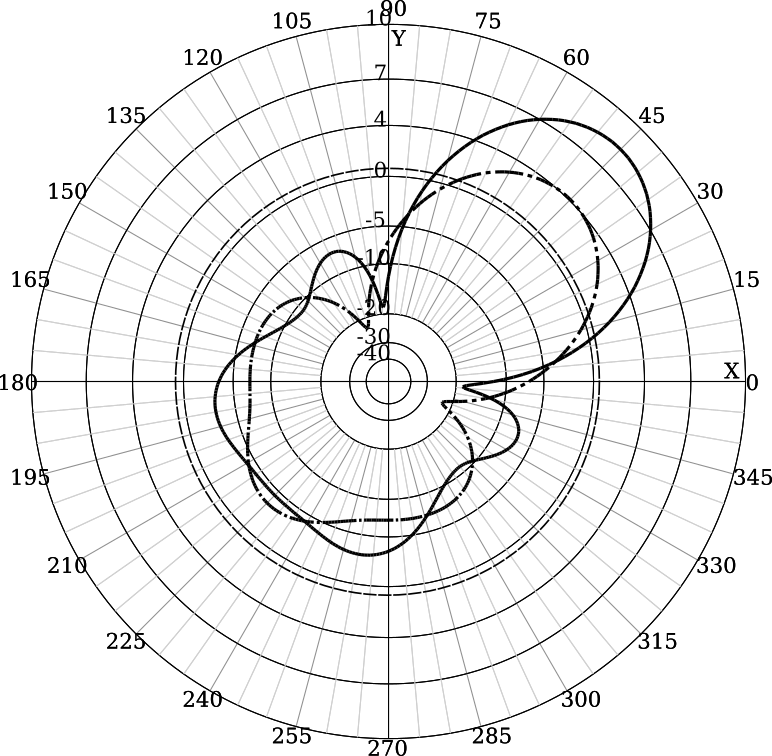
\includegraphics[width=1\linewidth]{r_bvd_20_results_h.png} \\ а)}
    \end{minipage}
    \hfill
    \begin{minipage}[h]{0.49\linewidth}
    \center{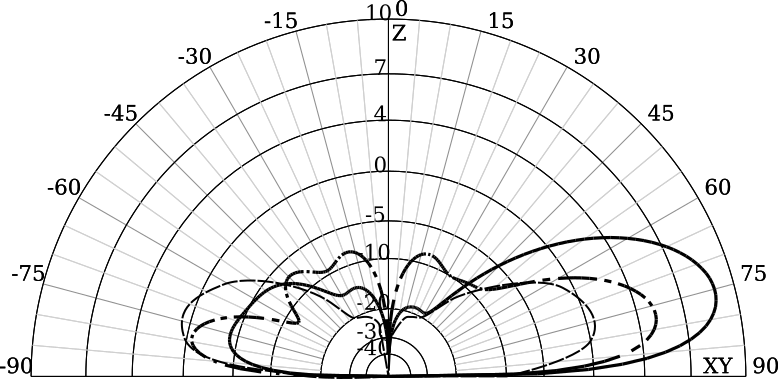
\includegraphics[width=1\linewidth]{r_bvd_20_results_v.png} \\ б)}
    \end{minipage}
    \caption{Горизонтальный (а) и вертикальный (б) план диаграммы направленности ШВД при расстоянии от центра излучателя до центра решетки 20 м. Пунктирной линией обозначено усиление одиночного излучателя, штрихпунктирной – простое фазирование, сплошной – решение задачи мат. программирования.}
    \label{pic:r_bvd_result}
    \end{figure}

\end{frame}
